\documentclass{beamer}

\usepackage{bookmark}
\usepackage{multicol}

\title{Deep Neural Network for Real-Time EEG Decoding of Musical Rhythm Imagery}
\author{Ir\'{a}n Rom\'{a}n}
\date{December 03, 2019}

\begin{document}
\setbeamertemplate{caption}{\raggedright\insertcaption\par}

\maketitle

\begin{frame}
	\frametitle{Pulse and Meter as Neural Resonance}
	
	\begin{itemize}

		\item Pulse: (aka beat) the repeating, periodic \textit{pulsation} 
			that we \textit{perceive} through time when we listen to music
		\begin{itemize}
			\item Tempo: the pulse's frequency over time
		\end{itemize}

		\item Meter: The patterns of accentuation between pulses (i.e. march or waltz)

		\item Neural Resonance: Music can trigger rhythmic bursts of high-frequency neural activity,
			 which may enable communication between auditory and motor cortices (Large \& Snyder 2009)

	\end{itemize}

\end{frame}

\begin{frame}
	\frametitle{Early EEG Evidence for Neural Resonance}

	Induced and evoked oscilatory activity reflect the processing and expectation of periodic stimuli

	\begin{figure}
		\centering
		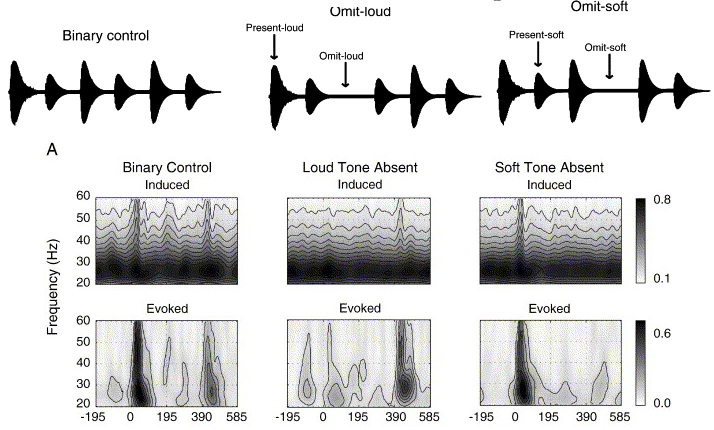
\includegraphics[scale=2.5]{fig1.png}
		\caption{Snyder \& Large 2005}
	\end{figure}

\end{frame}

\begin{frame}
	\frametitle{Pulse timing is reflected in beta- and gamma-bands}

	\begin{figure}
		\centering
		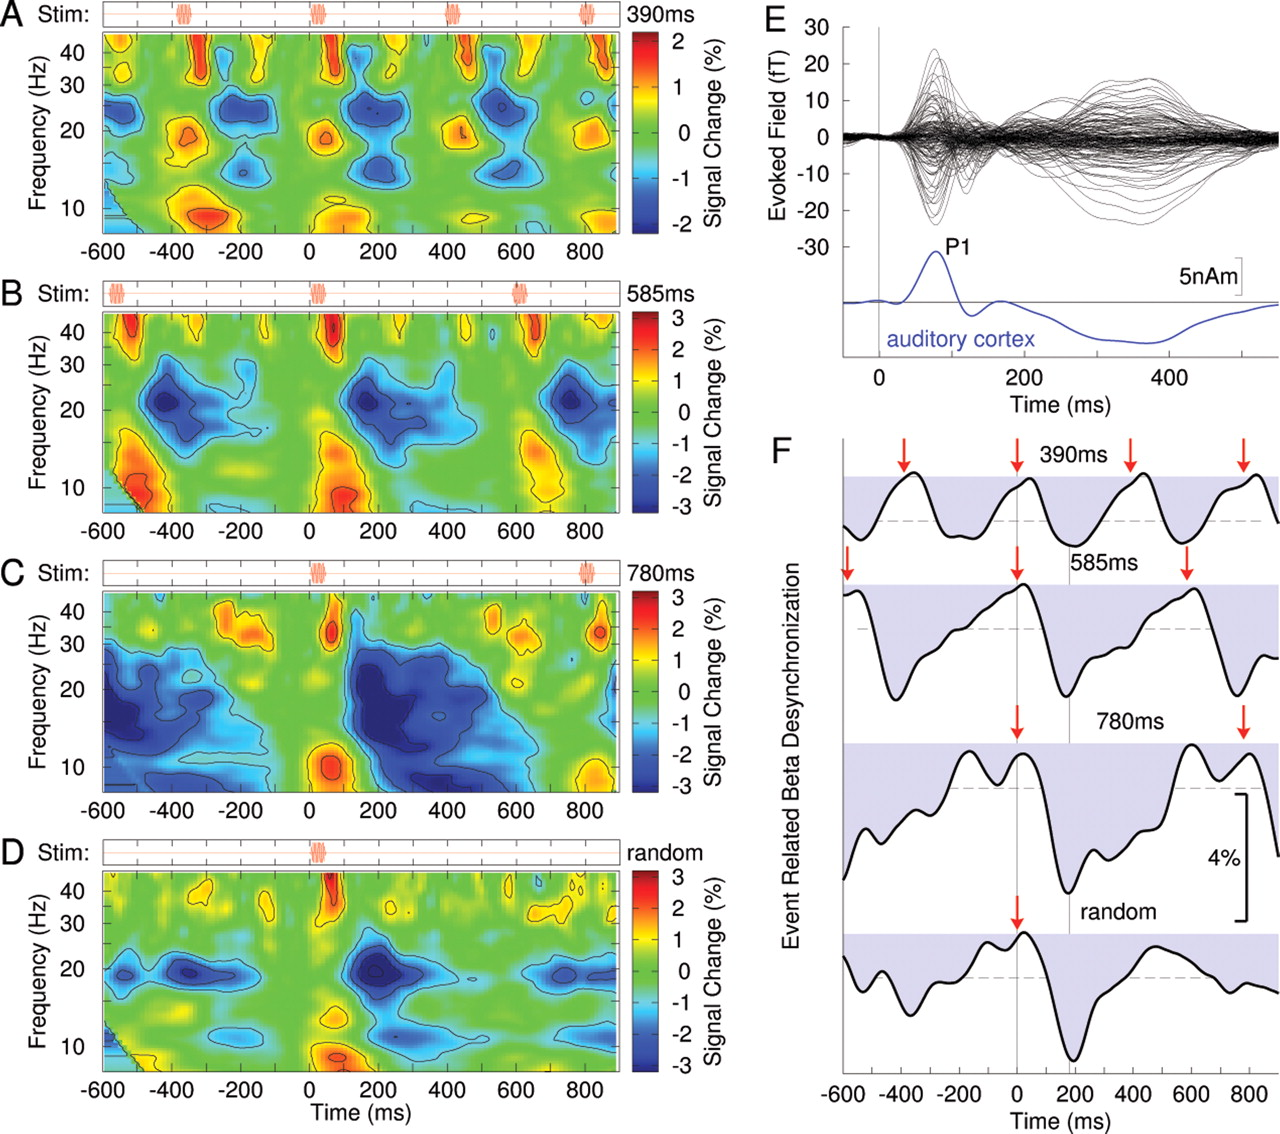
\includegraphics[scale=0.18]{fig5.jpg}
		\caption{Fujioka et al. 2009}
	\end{figure}

\end{frame}

\begin{frame}
	\frametitle{Pulse timing is reflected in beta- and gamma-bands}

	\begin{figure}
		\centering
		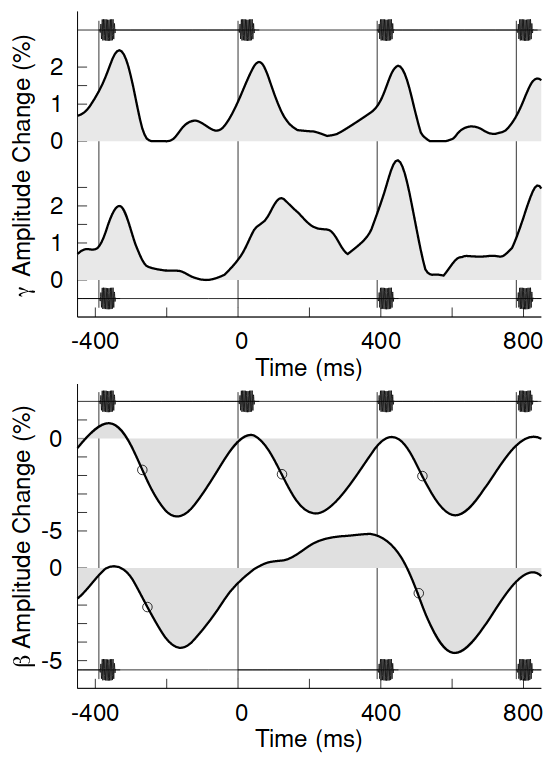
\includegraphics[scale=0.2]{fig2.png}
		\caption{Fujioka et al. 2012}
	\end{figure}

	This kind of analysis involves the averaging of hundreds of trials

\end{frame}

\begin{frame}
	\frametitle{Imagined meters are also reflected in the beta-band}

	Imagination of different meters (i.e. binary march vs ternary waltz) results in different beta-band patterns

	\begin{figure}
		\centering
		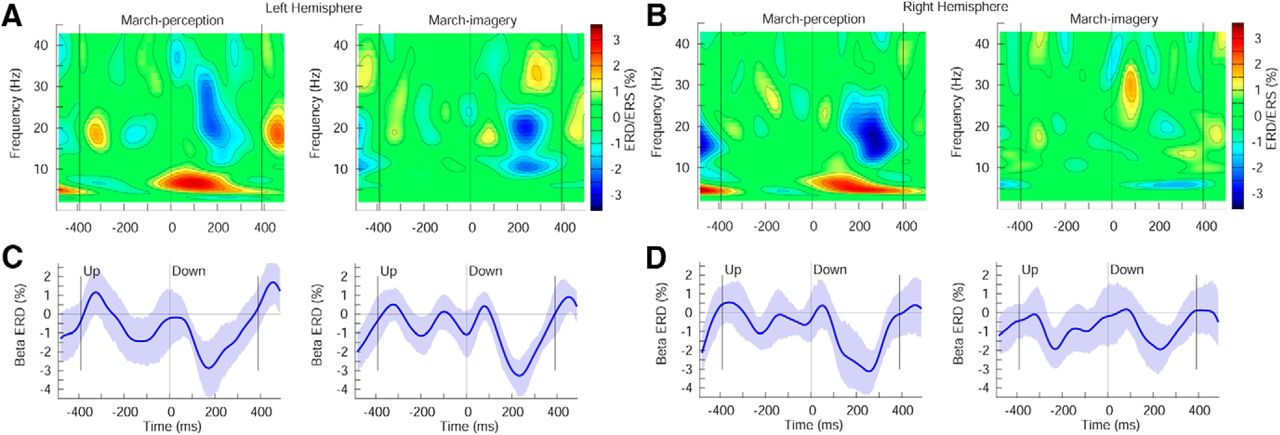
\includegraphics[scale=0.85]{fig3.jpg}
	\end{figure}
	\begin{figure}
		\centering
		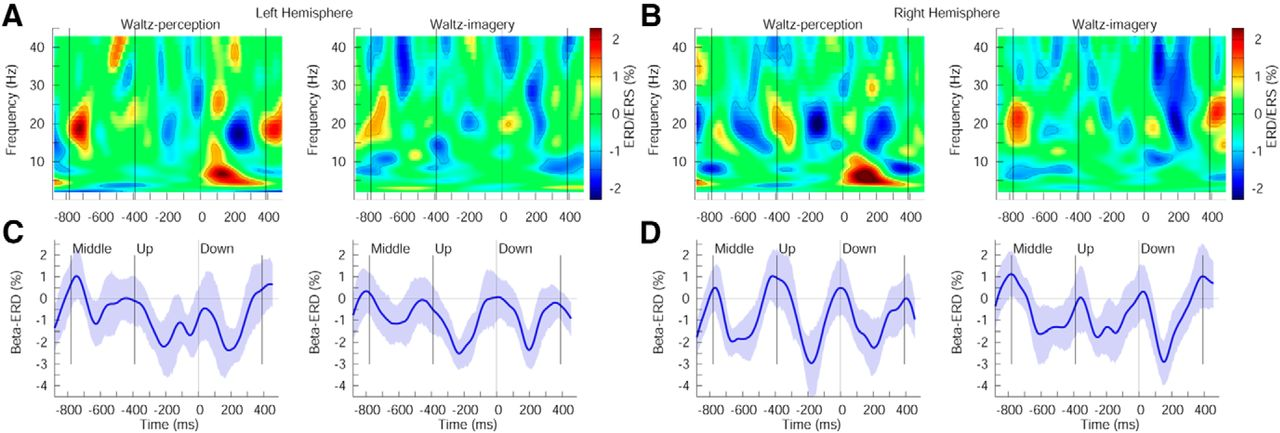
\includegraphics[scale=0.85]{fig4.jpg}
		\caption{Fujioka et al. 2015}
	\end{figure}

\end{frame}

\begin{frame}
	\frametitle{Primate oscillations reflect the metronome tempo}

	Dorsal putamen LFPs of macaques in a metronome tapping task	

	\begin{figure}
		\centering
			\item 
		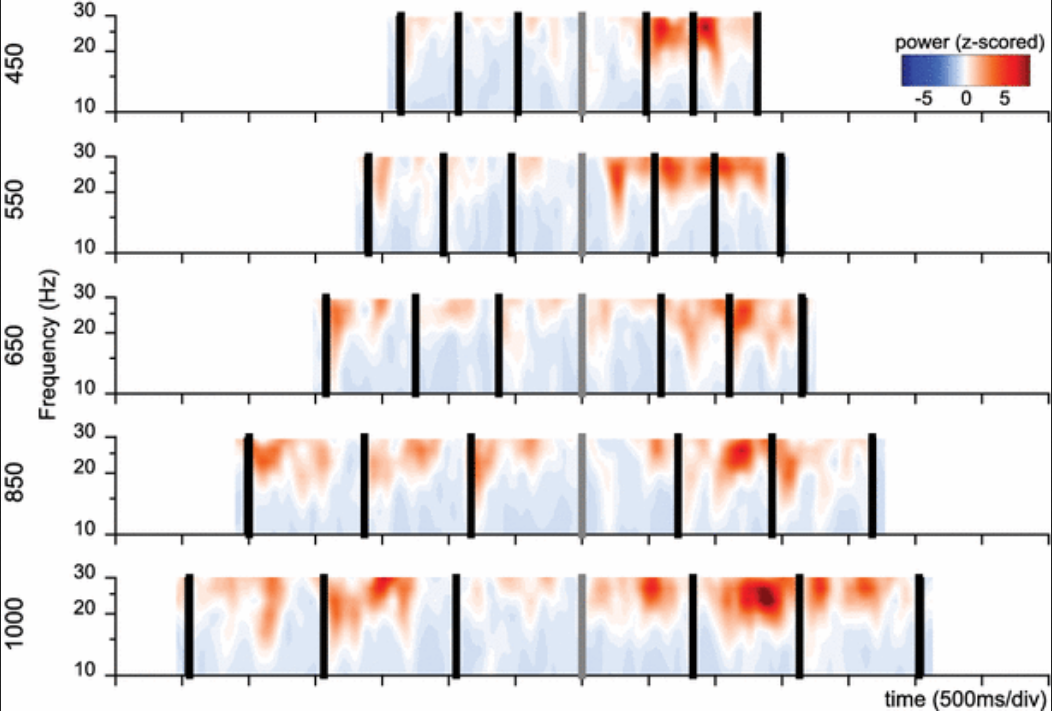
\includegraphics[scale=0.18]{fig6.png}
		\caption{Merchant \& Bartolo 2017}
	\end{figure}

	Bottomline: gamma reflects stimulus processing, while beta reflects the entrainment of large basal ganglia networks during internally driven pulse tapping

\end{frame}

\begin{frame}
	\frametitle{Research question and hypothesis}
	
	\begin{itemize}

		\item Pulse, tempo and meter can be observed in the neural correlates measured with EEG and MEG.

		\item To maximize the SNR, these observations require the analysis of hundreds of trials.

		\item \textbf{Research Question:} could these features be identified in single trials? and if so, can we decode from human brain data, in real-time, perceived and imagined musical features like pulse, tempo and meter? 
			 
		\item \textbf{Hypothesis:} Deep neural networks, like CNNs, can learn to identify these musical features on a single-trial level.

	\end{itemize}

\end{frame}

\begin{frame}
	\frametitle{Lit Review: What can CNNs learn from EEG data?}
	
	\begin{itemize}

		\item Individual subject classification with resting-state data (Ma et al. 2018)

		\item Motor imagery classification: left vs rigt hand (Tang et al. 2017)

		\item Motor imagery with Riemannian Geometry Classifiers (Barachant et al. 2011)

		\item Music imagery information retrieval (Tan et al. 2018)
		
		\item The key problem: domain adaptation and transfer learning (Lotte et al. 2018) 

	\end{itemize}

\end{frame}

\begin{frame}
	\frametitle{Individual subject classification (Ma et al. 2018)}
	
	\begin{itemize}

		\item Task: resting state with open and closed eyes

		\item CNN input: 64x160 EEG "images" 
		\begin{itemize}
			\item 64 EEG channels
			\item 1 second-long epochs ($fs = 160$)
			\item 50 (5) seconds of training (test) data per subject 
			\item 10 participants
		\end{itemize}

		\item CNN architecture: LeNet (6 channels in each conv layer)
	
		\item Performance: \textbf{88\% accuracy}

		\item Significance: 
		\begin{itemize}
			\item EEG for biometrics
		\end{itemize}

	\end{itemize}

\end{frame}

\begin{frame}
	\frametitle{Motor imagery classification: left vs right hand (Tang et al. 2018)}
	
	\begin{itemize}

		\item Task: imagination of right or left hand movements during 5 second trials (460 total)

		\item CNN input: 28x60 
		\begin{itemize}
			\item 28 EEG channels
			\item 3 seconds, 50ms fft frames (1 frequency band per subject)
			\item 350 (100) trials of traning (test) data per subject 
			\item 2 participants
		\end{itemize}
		
		\item CNN architecture
		\begin{figure}
			\centering
			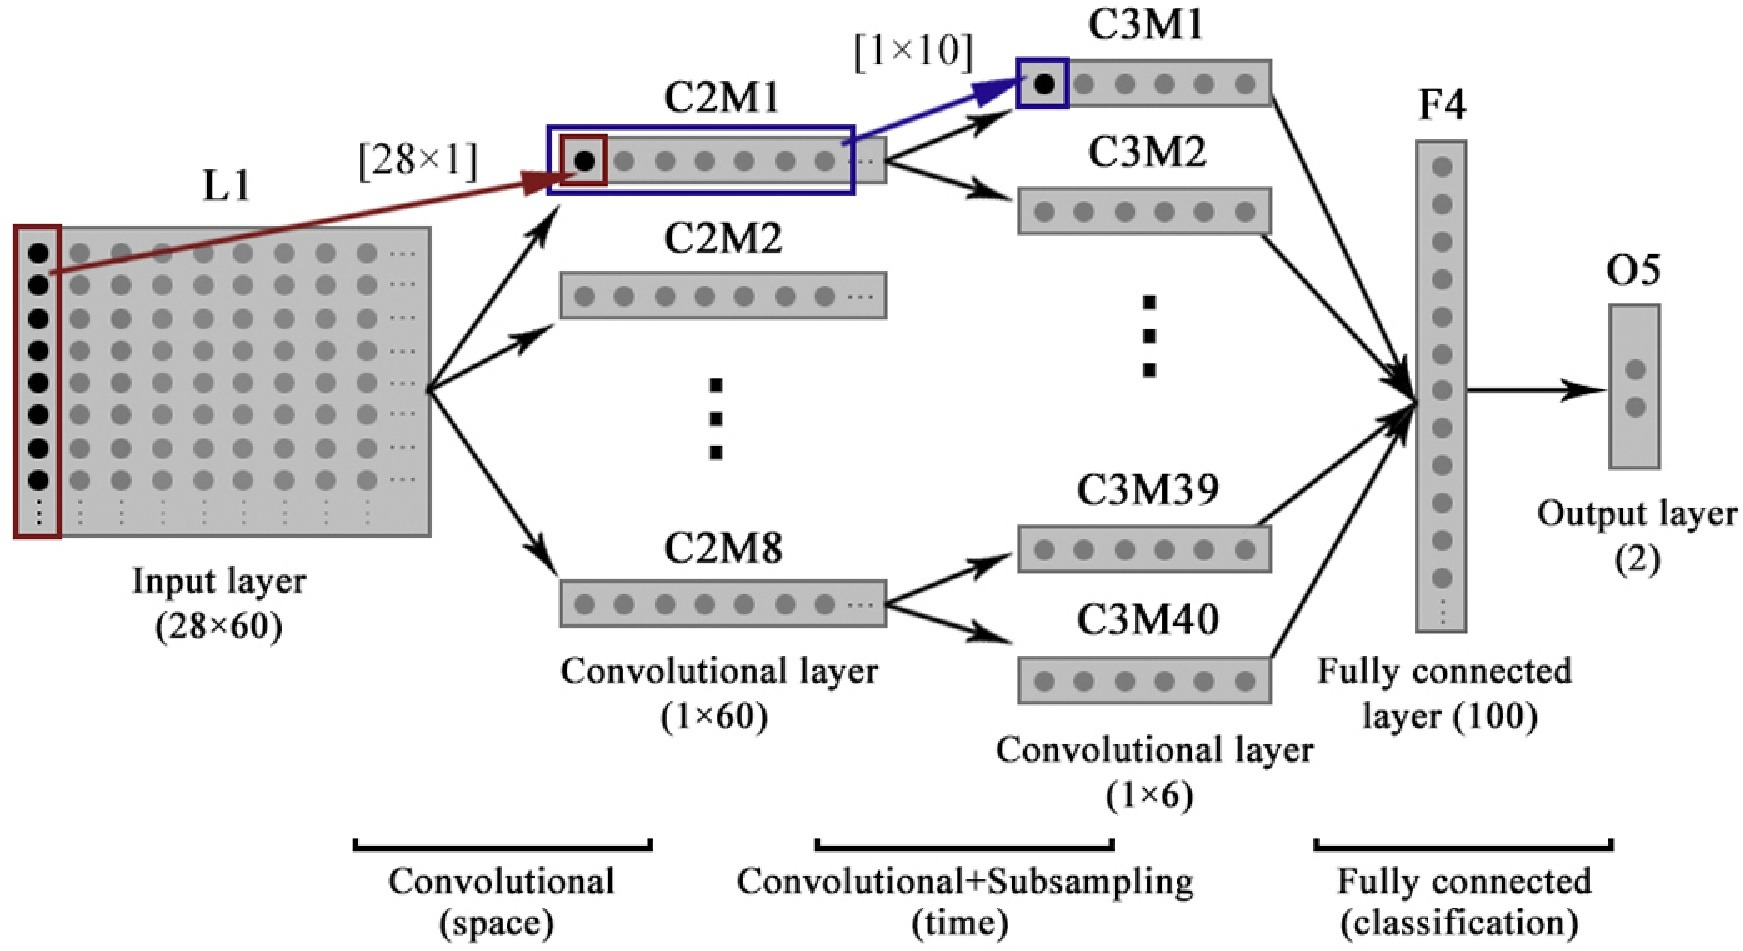
\includegraphics[scale=0.85]{fig7.jpg}
		\end{figure}
	
		\item Performance: \textbf{87\% accuracy}

		\item Significance: 
		\begin{itemize}
			\item Using CNNs to classify EEG with motor imagery
		\end{itemize}	

	\end{itemize}

\end{frame}

\begin{frame}
	\frametitle{Motor imagery with Rimennian Geometry Classifiers (Barachant et al. 2011)}
	
	\begin{itemize}

		\item Riemannian geometry studies smooth curved spaces that can be locally and linearly approximated with tangents
		
		\item Assumption: each EEG mental state has different power and spatial distribution

		\item The covariance matrix of the EEG data can code this information
		\begin{figure}
			\centering
			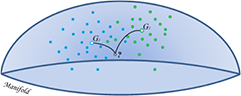
\includegraphics[scale=1.0]{fig8.jpg}
		\end{figure}

		\item Performance: \textbf{70\% accuracy} in a four-class, motor imagery task (four extremities)

		\item Significance: 
		\begin{itemize}
			\item This method is considered to be the \textit{state-of-the-art} (Lotte et al. 2018)
		\end{itemize}	

	\end{itemize}

\end{frame}


\begin{frame}
	\frametitle{Music imagery information retrieval (Tan et al. 2018)}
	
	\begin{itemize}

		\item OpenMIIR dataset: listening and imagination of 12 known musical stimuli (Stober et al. 2015)

		\item CNN input: raw EEG signal 
		\begin{itemize}
			\item 64 EEG channels
			\item 240 trials per participant (12 stimuli x 4 conditions x 5 blocks). Avg trial length (\~10 sec)
			\item 10 participants
		\end{itemize}
		
		\item CNN architecture
		\begin{figure}
			\centering
			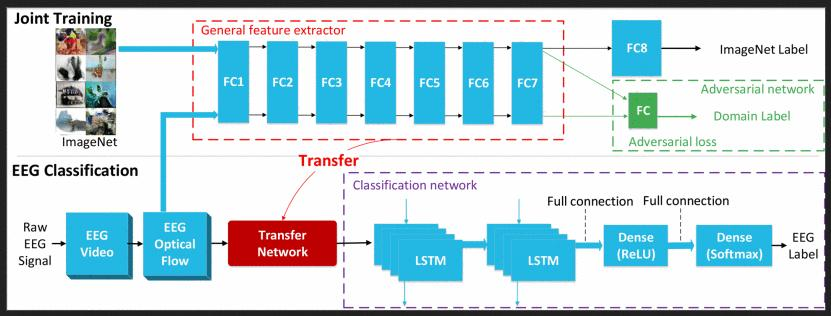
\includegraphics[scale=0.85]{fig9.jpg}
		\end{figure}
	
		\item Performance:
		\begin{figure}
			\centering
			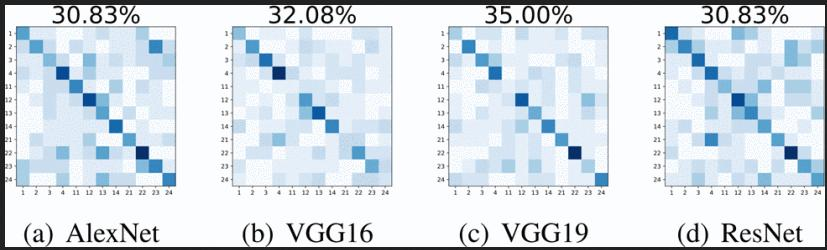
\includegraphics[scale=0.85]{fig10.jpg}
		\end{figure}
	
		\item Significance:
		\begin{itemize}
			\item Deep transfer learning exploiting EEG \textit{multimodality} and using joint training for knowledge transfer.
		\end{itemize}	
	
	\end{itemize}

\end{frame}

\begin{frame}
	\frametitle{The key problem: domain adaptation and transfer learning (Lotte et al. 2018)}
	
	\begin{itemize}

		\item In EEG, major changes in data distribution can occur between subjects or across time.

		\item Solution: transfer learning (calibration) to optimize the algorithm across time and across subjects

		\begin{itemize}
			\item Learn the transformation that explains the change in the data distribution
			\item Reweighting
			\item Find the common features between the two distributions
		\end{itemize}

	\end{itemize}

\end{frame}



\begin{frame}
	\frametitle{Research question and hypothesis}
	
	\begin{itemize}

		\item Pulse, tempo and meter can be observed in the neural correlates measured with EEG and MEG.

		\item To maximize the SNR, these observations require the analysis of hundreds of trials.

		\item \textbf{Research Question:} could these features be identified in single trials? and if so, can we decode from human brain data, in real-time, perceived and imagined musical features like pulse, tempo and meter? 
			 
		\item \textbf{Hypothesis:} Deep neural networks, like CNNs, can learn to identify these musical features on a single-trial level.

	\end{itemize}

\end{frame}

\begin{frame}
	\frametitle{Methods: EEG dataset task}
	
	\begin{figure}
		\centering
		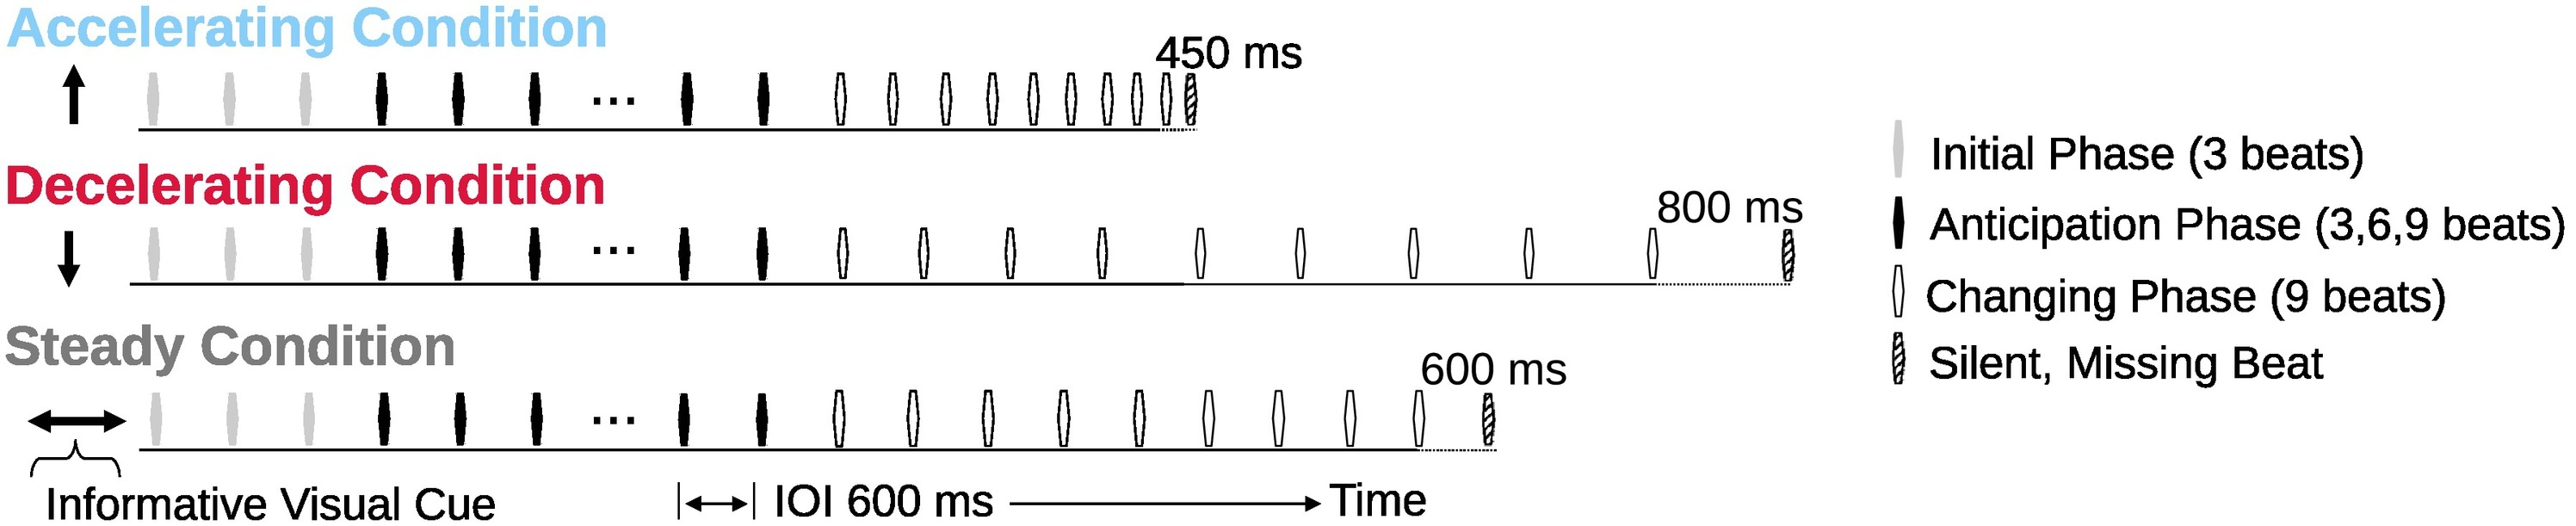
\includegraphics[scale=0.85]{fig11.jpg}
	\end{figure}
	
	\begin{itemize}

		\item 21 Participants listened 450 trials, each consisting of \~18 metronome clicks that either:
		\begin{itemize} 
			\item accelerate
			\item decelerate
			\item remain isochronous
		\end{itemize}

		\item The metronome starts at 1.67Hz (600ms inter-stimulus-interval)

		\item The three types of trials are equally likely to appear and are presented randomly.

		\item Stimuli presentation was evenly divided across eight blocks

		\item At the beginning of each trial, participants see a visual cue that tells them what the metronome will do. 
		
		\item No behavioral task related to metronome rate changes.

	\end{itemize}

\end{frame}

\begin{frame}
	\frametitle{Methods: EEG equipment}
	
	\begin{itemize}

		\item 64 channel Neuroscan

		\item 500Hz sampling rate

		\item 2 electro-oculogram channels to record horizontal and vertical eye movements 
		
		\item Insert earphones and a monitor delivered the stimuli

	\end{itemize}

\end{frame}

\begin{frame}
	\frametitle{Methods: EEG data processing}
	
	\begin{itemize}

		\item 10 noisy EEG channels were eliminated from all recordings.
		
		\item The noisy EEG channels were at the edge of the EEG cap.

		\item Eye movement artifacts were removed using the signal-space projection method. 

		\item 200ms epochs were calculated starting 16ms before each click or visual cue.

		\item Epochs were baseline corrected with the mean of the eeg amplitude before each click (100ms).

		\item Epochs were downsampled from 500Hz to 125Hz sampling rate.
	
		\item Rejected epochs with EEG peak-to-peak difference greater than 100$\mu$V in any channel.

	\end{itemize}

\end{frame}

\begin{frame}
	\frametitle{Methods: CNN input data}
	
	\begin{itemize}

		\item 10\% of all epochs were held-out as validation data
		\begin{itemize}
			\item 133,813 training epochs (7,363 visual epochs)
			\item 14,791 validation epochs (803 visual epochs)
		\end{itemize}

		\item \~6,300 epochs per participant (21 total)
	
		\item Epochs were multiplied by $10^6$ and cast to be float32

		\item Data shape is: \texttt{[None, 54, 1, 25]}

	\end{itemize}

	\begin{figure}
		\centering
		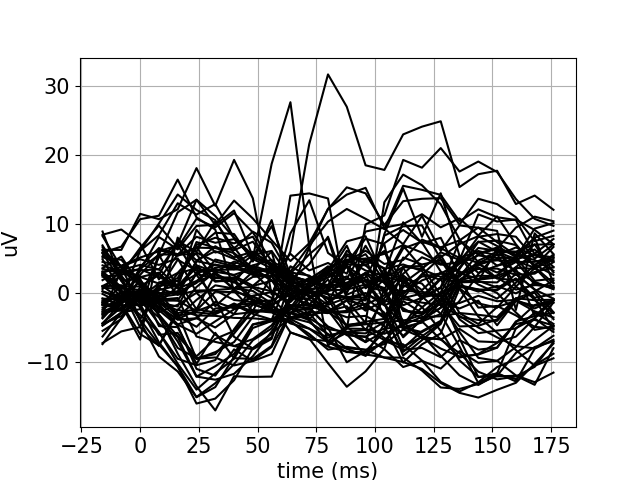
\includegraphics[scale=0.85]{fig12.png}
	\end{figure}

\end{frame}

\begin{frame}
	\frametitle{Methods: LeNet architecture}

	\begin{figure}
		\centering
		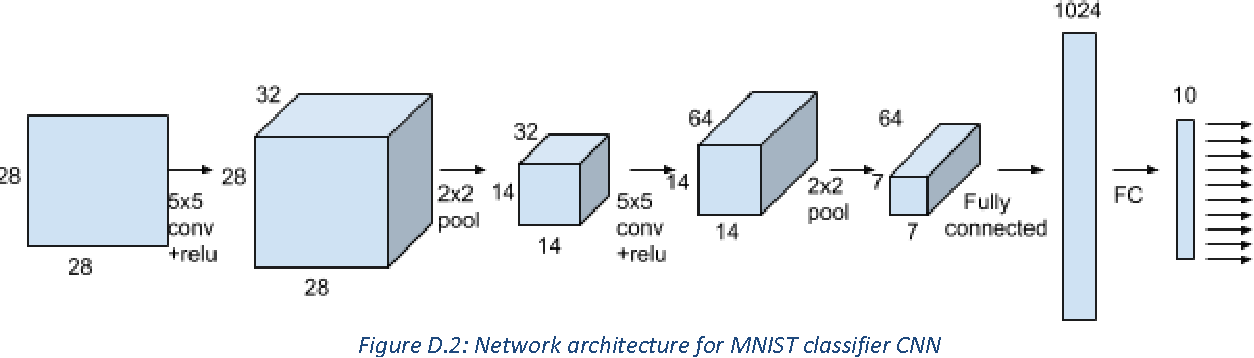
\includegraphics[scale=0.85]{fig13.png}
	\end{figure}
	
\end{frame}

\begin{frame}
	\frametitle{Methods: EEG classification experiments}

	\begin{itemize}
		
		\item Subject classification 

		\item Audio vs visual stimulus classification

		\item Accelerating vs decelerating vs steady beat classification

	\end{itemize}

\end{frame}

\begin{frame}
	\frametitle{Results: Subject classification}

	\begin{itemize}
		
		\item \textbf{90\% accuracy}

		\item Trained with pulse epochs (no visual stimuli epochs) 

		\item Confusion matrix
		\begin{figure}
			\centering
			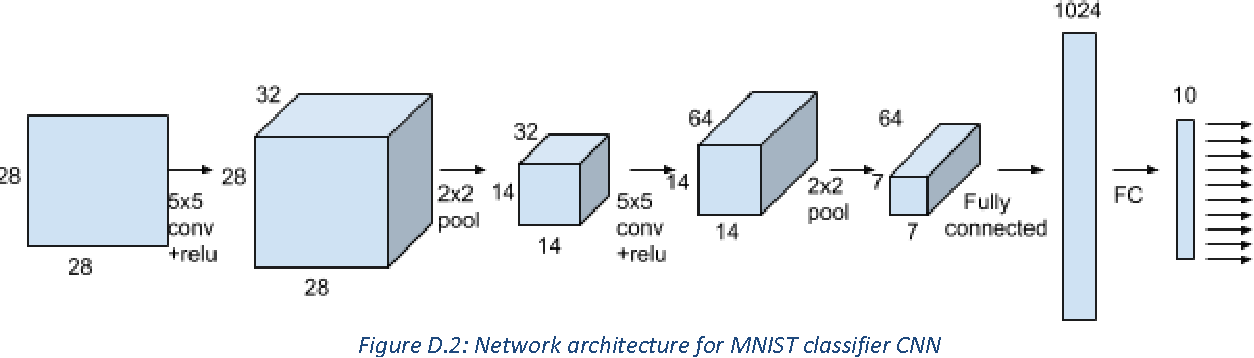
\includegraphics[scale=1.0]{fig13.png}
		\end{figure}
	\end{itemize}

\end{frame}

\begin{frame}
	\frametitle{Results: Audio vs visual stimulus classification}

	\begin{multicols}{2}
		Accuracy per Participant
		\begin{tabular}{l|l}
			P1 & 0.98 \\
			P2 & 0.82 \\
			P3 & 0.90 \\
			P4 & 0.85 \\
			P5 & 0.94 \\
			P6 & 0.78 \\
			P7 & 0.91 \\
			P8 & 0.94 \\
			P9 & 0.87 \\
			P10 & 0.86 \\
			P11 & 0.94 \\
			P12 & 0.99 \\
			P13 & 0.95 \\
			P14 & 0.88 \\
			P15 & 0.92 \\
			P16 & 0.93 \\
			P17 & 0.74 \\
			P18 & 0.86 \\
			P19 & 0.93 \\
			P20 & 0.83 \\
			P21 & 0.87 \\
		\end{tabular}
		\columnbreak

	\end{multicols}

\end{frame}

\end{document}
